\documentclass[tikz,border=2pt]{standalone}
\usepackage{amsmath}
\usepackage{pgfplots}
\pgfplotsset{compat=1.18}
\usetikzlibrary{arrows.meta}
\begin{document}
% Conditional variance against mean: Poisson mu, quasi-Poisson 1.5 mu, negative binomial mu + mu^2/4 (r = 4);
% both overdispersed models give variance 3 at mu = 2 but differ elsewhere.
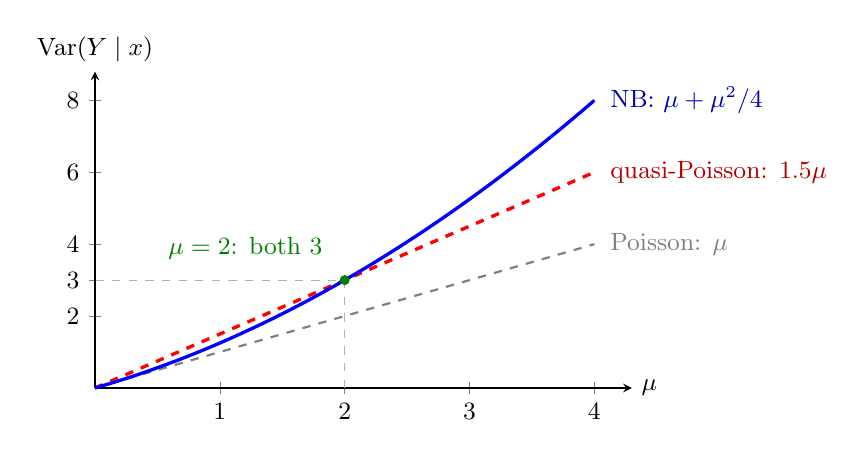
\begin{tikzpicture}[font=\small, >={Latex[length=2mm]}]
  \begin{axis}[
    axis lines=left, xmin=0, xmax=4.3, ymin=0, ymax=8.8,
    xtick={1,2,3,4}, ytick={2,3,4,6,8},
    xlabel={$\mu$}, ylabel={$\operatorname{Var}(Y\mid x)$},
    xlabel style={at={(axis description cs:1,0)}, anchor=west},
    ylabel style={rotate=-90, at={(axis description cs:0,1)}, anchor=south},
    samples=80, width=8.4cm, height=5.6cm, clip=false]
    \addplot[gray, thick, dashed, domain=0:4] {x};
    \addplot[red, very thick, dashed, domain=0:4] {1.5*x};
    \addplot[blue, very thick, domain=0:4] {x+x^2/4};
    \draw[gray!60, thin, dashed] (axis cs:2,0) -- (axis cs:2,3) -- (axis cs:0,3);
    \fill[green!50!black] (axis cs:2,3) circle (1.8pt);
    \node[green!50!black, anchor=south east] at (axis cs:1.9,3.3) {$\mu=2$: both $3$};
    \node[blue!70!black, anchor=west] at (axis cs:4.05,8) {NB: $\mu+\mu^2/4$};
    \node[red!70!black, anchor=west] at (axis cs:4.05,6) {quasi-Poisson: $1.5\mu$};
    \node[gray, anchor=west] at (axis cs:4.05,4) {Poisson: $\mu$};
  \end{axis}
\end{tikzpicture}
\end{document}
